\section{Topic Tree}

\subsection{Home Page}

From the homepage, a user (both students and academics) can get to the topic tree from the sidebar.\\

\begin{figure}[h!]
    \centering
    
\includegraphics[scale=0.4]{topic-tree-dashboard}
    \caption{Topic Tree Link in Dashboard}
\end{figure}

This allows quick access to the topic tree so students can easily view which topics they must complete next and academics can also easily edit topics and upload content.\\

\subsection{Graph View}

\textbf{Design} \\

The main feature of the topic tree is the graph view. Here the user can view the topic groups, topics and how each topic is related to each other (through prerequisites). On first load, the topic groups are shown with arrows to indicate the prerequisites. In the below screenshot, there is a topic in Programming Fundamentals that is a prerequisite for a topic in C++ Programming i.e. a student must complete the topic in Programming Fundamentals before they can start topics in C++ Programming.\\

\begin{figure}[h!]
    \centering
    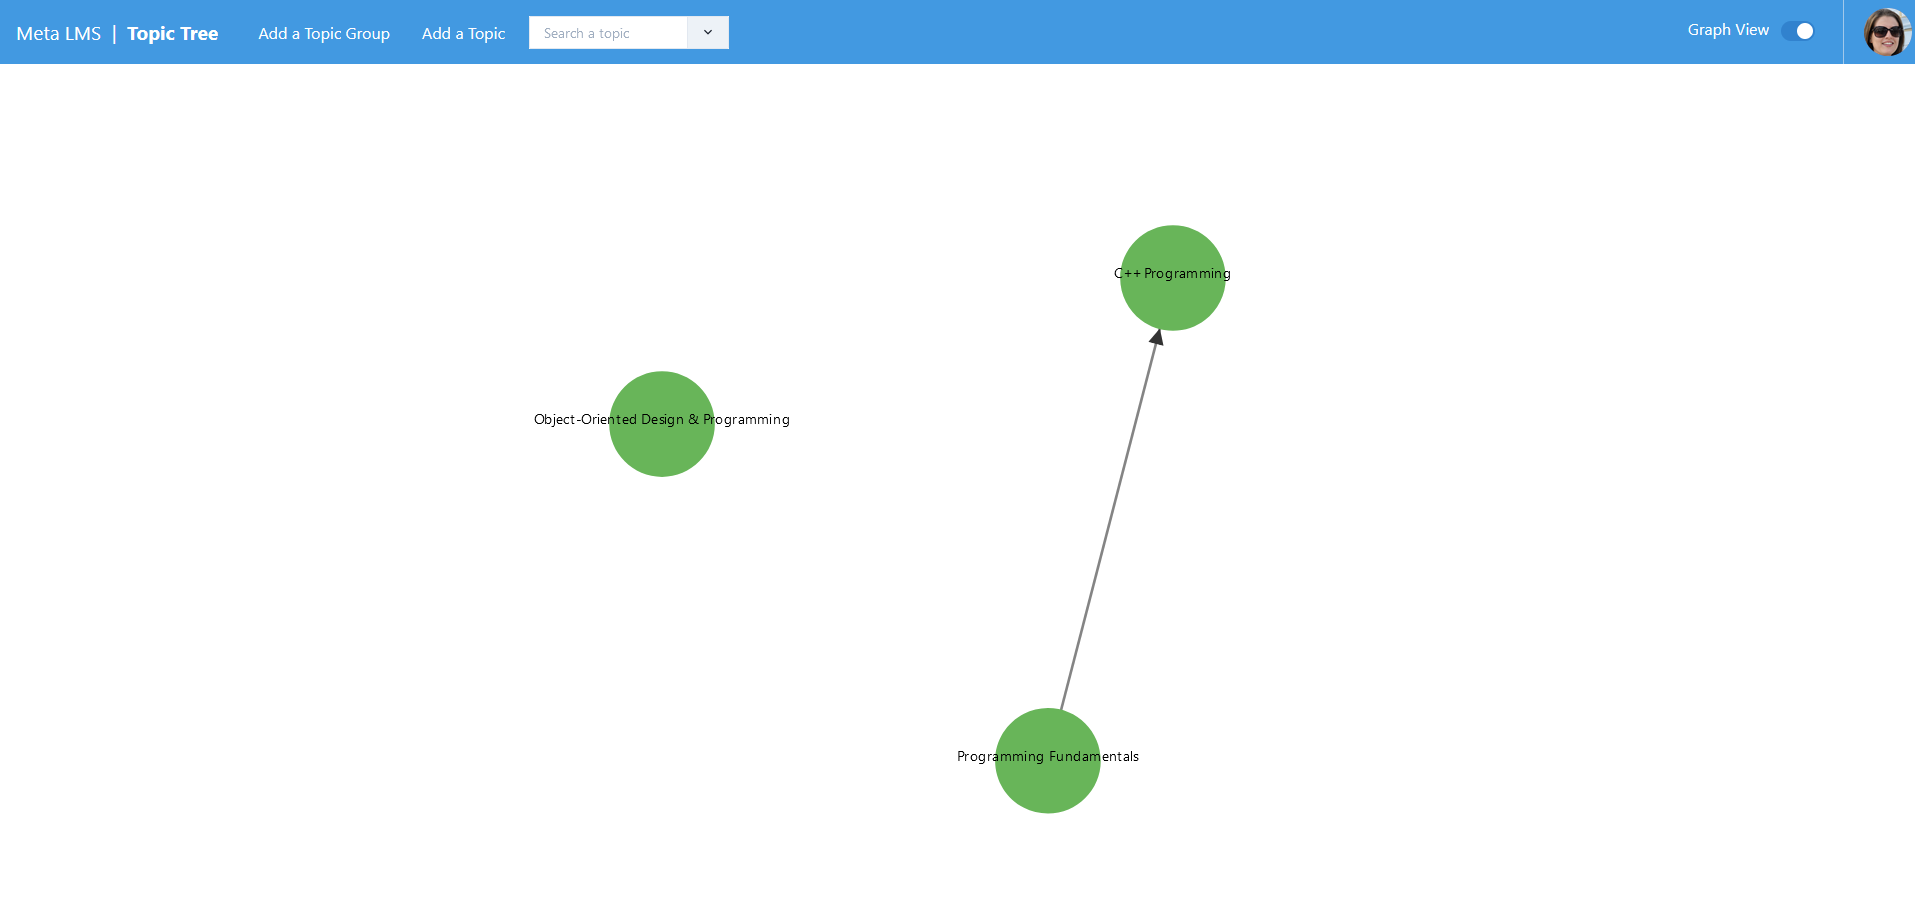
\includegraphics[scale=0.3]{topic-tree-graph-view-actual}
    \caption{Topic Tree Graph View}
\end{figure}

A topic group is marked as green, and when clicked it expands into the individual topics as shown below. \\

\begin{figure}[h!]
    \centering
    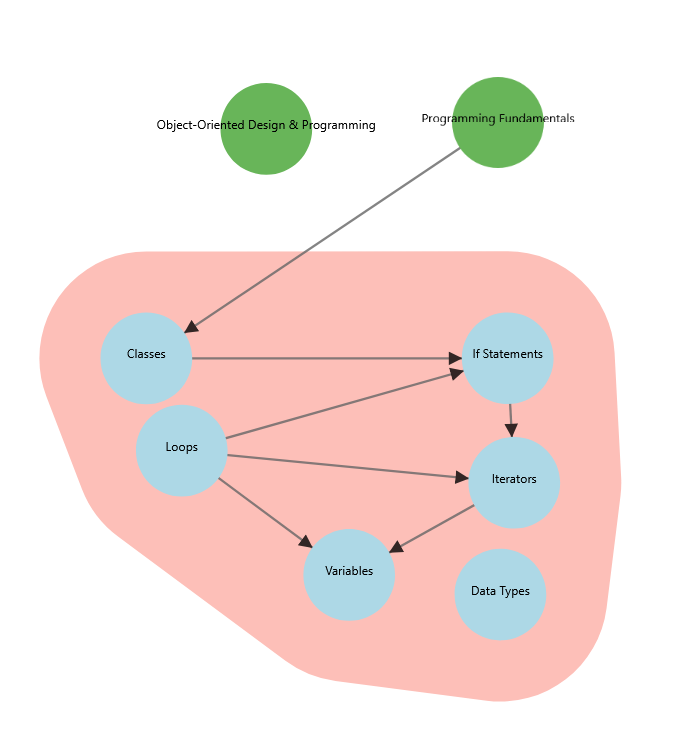
\includegraphics[scale=0.4]{topic-tree-expanded}
    \caption{Topic Tree Expanded}
\end{figure}

A hull around the topics is drawn to indicate that they are part of the same topic group, as in the above example the topics are part of C++ Programming.\\

\begin{figure}[h!]
    \centering
    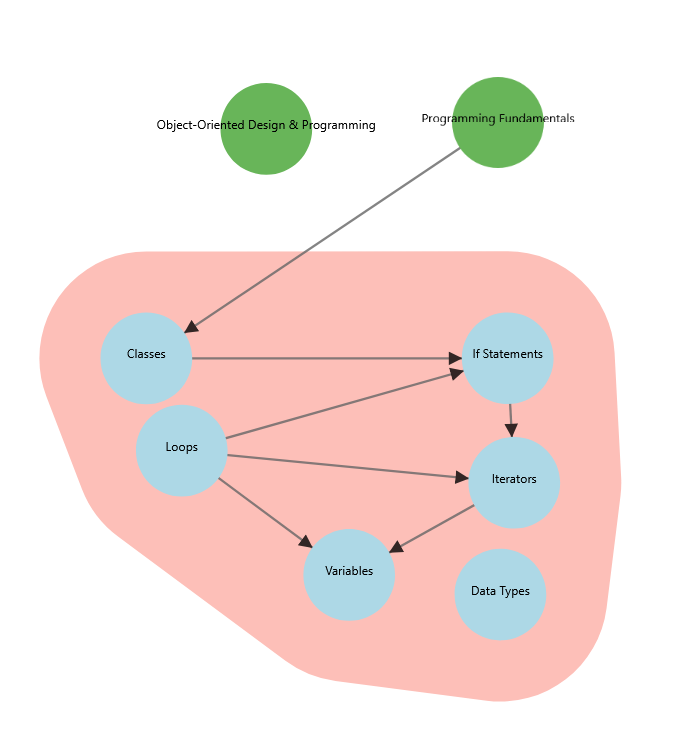
\includegraphics[scale=0.4]{topic-tree-hull}
    \caption{Topic Tree - Hull}
\end{figure}

The graph can be zoomed in, and you can drag topics out to make topics to be more visible. 

\textbf{Purpose} \\

The topic tree graph view allows users to view the relationship between topics and topic groups. Users can easily see which topics are the prerequisites of which other topics, and view the topics inside topic groups. This simplifies reusability for academics, as they can choose topics to add as prerequisites to their own topics.

\textbf{What was implemented} \\
The main graph view has been implemented as shown above. Features include clicking a topic group to expand into the topics inside it, showing the relationship between topics, and outlining the topics inside a topic group with a hull i.e. shape around the topics.

\textbf{How it was implemented} \\
D3 was used as a library to display the graph view. The list of topics with their topic groups is loaded from the database, and D3 algorithms are applied to create the hull, topic groups and topics on the graph.


\subsection{List View}


Some users may want to view the topics in a list instead of a graph.\\

\textbf{Design} \\

\begin{figure}[h!]
    \centering
    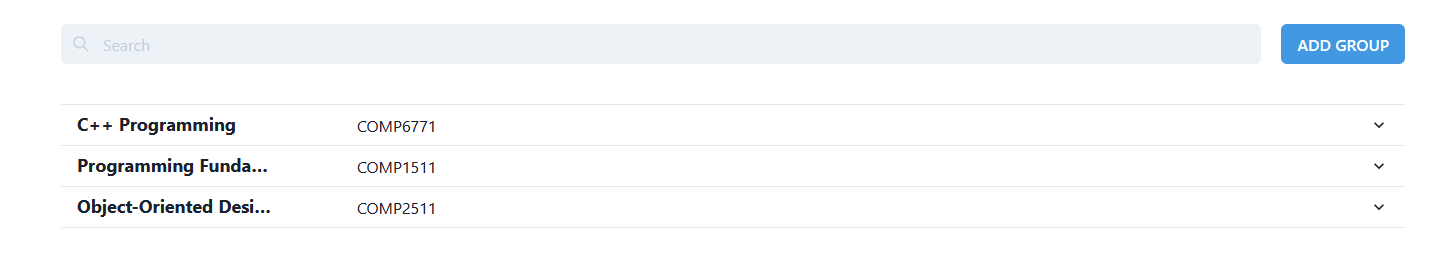
\includegraphics[scale=0.4]{topic-tree-list-actual}
    \caption{Topic Tree - List View}
\end{figure}

A list of the various topic groups is viewable, and when a topic group is clicked, the topics that are in the topic group expands as shown below.\\

\begin{figure}[h!]
    \centering
    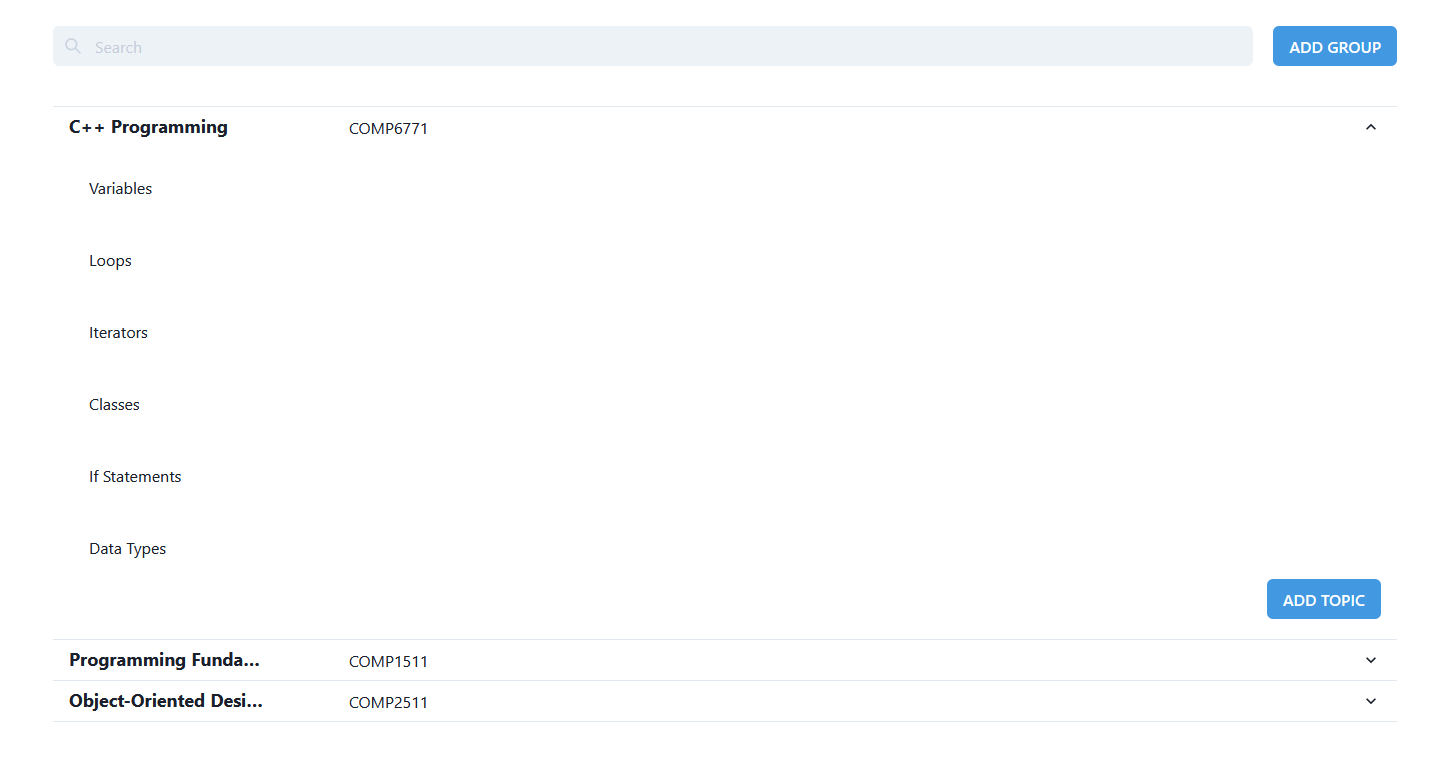
\includegraphics[scale=0.4]{topic-tree-list-expanded}
    \caption{Topic Tree - List View Expanded}
\end{figure}

\textbf{Purpose} \\
The purpose of this view is to allow academics and users to view the topics in a simpler view if they wish. Some users may find the graph view too confusing to use or not as efficient when searching for topics, and so the list view provides an alternative to the graph view. As discussed in the analysis section, potential users reported that having the choice between the two views was a good feature of the topic tree.\\

\textbf{What was implemented} \\
Users can view the topic groups in list form, and click a topic group to view the relevant topics. A search bar is viewable at the top of the list view, to allow users to search for their topic or topic group.\\

\textbf{How it was implemented} \\
Chakra UI components were used to design the list view. The same endpoint as the graph view was used to load the topic groups and topics, and several React features were used to implement searching.

\subsection{Resources}

When a topic is clicked on the graph view or the list view, the user can then view the prerequisites of that topic, tags for search optimisation, and any files associated with the topic.

\begin{figure}[h!]
    \centering
    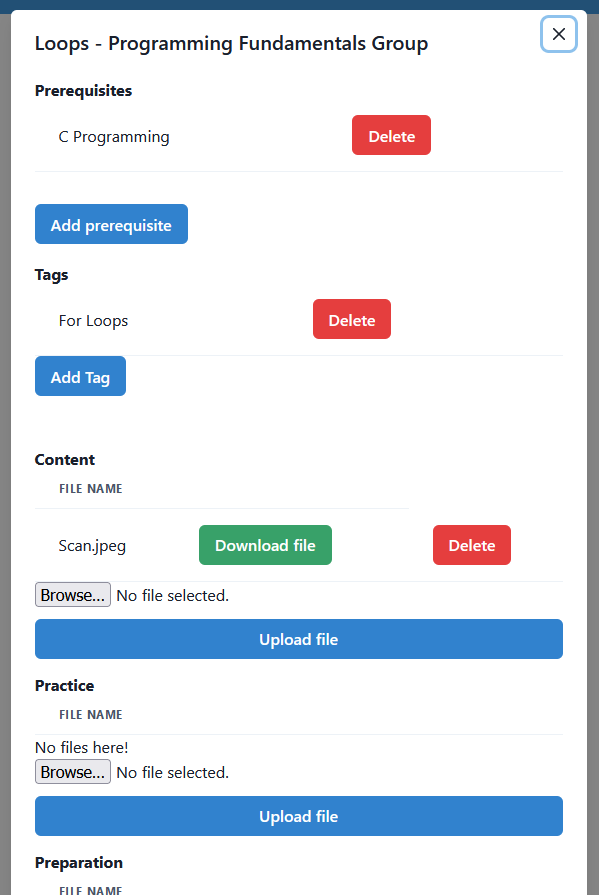
\includegraphics[scale=0.4]{topic-tree-view-resource}
    \caption{Topic Tree - View Resource}
\end{figure}

There are four file sections: Content, Practice, Preparation and Assessments. This is so it is adaptable to most learning models. Academics can upload any file they would like to a topic, and it will be viewable for all to view. In the future, permissions will be implemented to restrict access to certain resources. Third party integration with services such as YouTube, Echo360 and The Box will also be added.\\

\begin{figure}[h!]
    \centering
    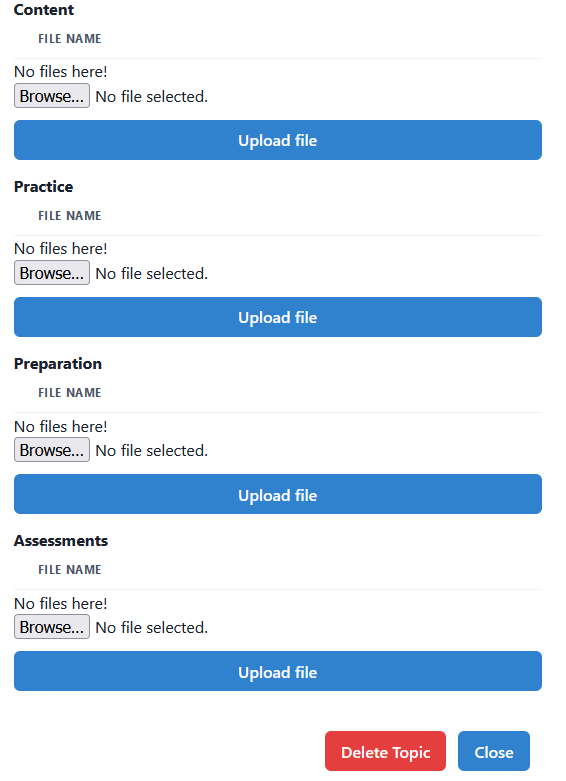
\includegraphics[scale=0.4]{topic-tree-file-sections}
    \caption{Topic Tree - File Sections}
\end{figure}

\textbf{Purpose} \\
The purpose of the resources modal is to allow users to view files and edit prerequisites and tags. This makes it easier for users to add or remove files, and makes it possible to edit the topic tree itself.\\

\textbf{What was implemented} \\
Users can view, add and delete prerequisites, as well as tags and files. Students are put in a view only state, where they cannot edit, delete or add prerequisites, tags or files.\\

\textbf{How it was implemented} \\
This modal was implemented using Chakra UI's modal library. Topic details such as files are taken from the original backend request when the topic tree is loaded, and POST and PUT requests are made when prerequisites, tags and files are edited.

\subsection{Adding topics and topic groups}
Users can also add a topic to a topic group, and add prerequisites to this topic in the same popup window. \\

\textbf{Design} \\

\begin{figure}[h!]
    \centering
    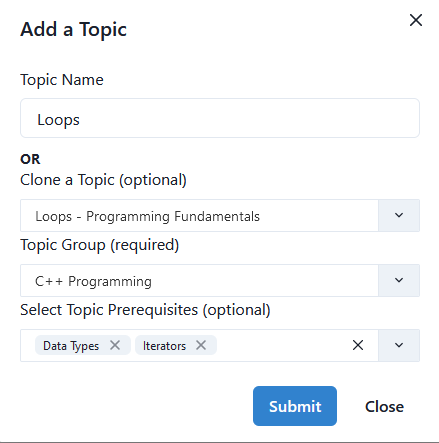
\includegraphics[scale=0.4]{topic-tree-add-topic-modal}
    \caption{Topic Tree - Add Topic}
\end{figure}

Users can also clone a topic i.e. if there is a topic in another topic group, academics can clone the materials in that topic and put it into another topic group. \\

Academics can also add topic groups, and search for a topic in the search bar in the header. Tags can be assigned to a topic which users can search for in the search bar to improve searchability of topics.

\begin{figure}[h!]
    \centering
    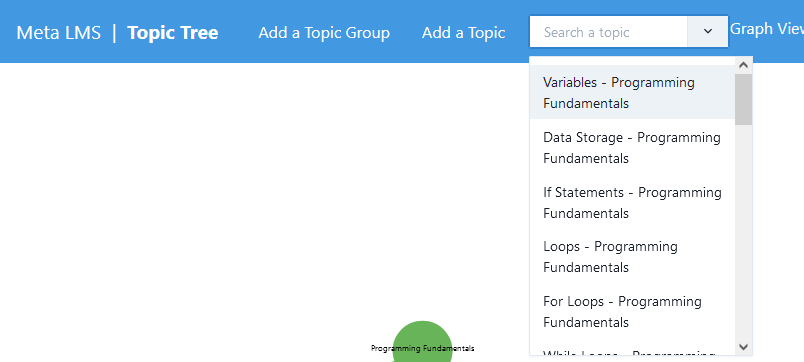
\includegraphics[scale=0.4]{topic-tree-search}
    \caption{Topic Tree - Search Bar}
\end{figure}

\textbf{Purpose} \\
Academics (not students) can add topics and topic groups to the topic tree, to allow further editing capability to the topic tree. The cloning feature also furthers reusability, allowing academics to clone topics and their respective materials into their own topic group.

\textbf{What was implemented} \\
Users can type a new name of their topic group into the add topic group window to create a new topic group. Users can also select prerequisites when creating a new topic, or select an existing topic to clone. \\

\textbf{How it was implemented} \\
Similar to previous modals, Chakra UI was used to create the topics and topic groups. POST end points were set up so when a new topic or topic group is created, POST requests are sent to the server to add new entries to the database.